\subsection{Reuniones}

  \subsubsection{Listar}

  \paragraph{}La aplicación permite generar el listado de las reuniones del
  alumno que ha accedido a la aplicación, para un determinado curso
  académico. Se puede ver una captura de pantalla de este listado en la figura
  \ref{capturaPantallaListaReuniones}.

  \begin{figure}[!ht]
    \begin{center}
      \fbox{
      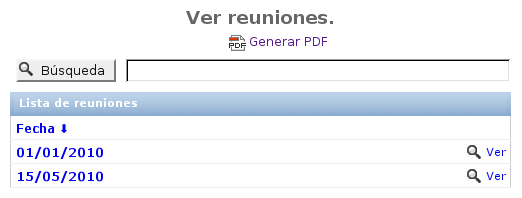
\includegraphics[scale=0.55]{4.Funcionamiento_Aplicacion/4.3.Gestion/4.3.4.Alumno/4.3.4.4.Reunion/lista_reuniones.png}
      }
      \caption{Captura de pantalla de la lista de reuniones para el usuario \textit{Alumno}.}
      \label{capturaPantallaListaReuniones}
    \end{center}
  \end{figure}

  \subsubsection{Ver reunión}

  \paragraph{}Si pulsamos en la fecha de la reunión, o en el icono \textit{Ver}
  del listado de reuniones, accederemos a ver la información específica de dicha
  reunión, así como las posibles preguntas que haya realizado el asesor. Esta
  pantalla es la que muestra la figura \ref{capturaPantallaVerReunion}.

  \begin{figure}[!ht]
    \begin{center}
      \fbox{
      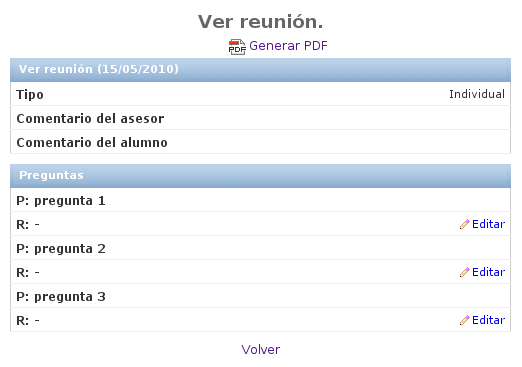
\includegraphics[scale=0.55]{4.Funcionamiento_Aplicacion/4.3.Gestion/4.3.4.Alumno/4.3.4.4.Reunion/ver_reunion.png}
      }
      \caption{Captura de pantalla de la vista de una reunión para el usuario \textit{Alumno}.}
      \label{capturaPantallaVerReunion}
    \end{center}
  \end{figure}
